\documentclass{beamer}
\usepackage[utf8]{inputenc}
\usepackage[T1]{fontenc}
\usepackage[english]{babel}
\usepackage{amssymb}
\usepackage{verbatim}
\usepackage{beamerthemesplit}
\usepackage{graphicx}
\usepackage{figlatex}
\usepackage{minted}

\beamertemplatetransparentcovereddynamic

\usecolortheme{progressbar}
\usefonttheme{progressbar}
\useoutertheme{progressbar}
\useinnertheme{progressbar}

\graphicspath{{figures/}}

\title{Layers for OpenCL}
\author{Brice Videau (Argonne National Laboratory)}

\begin{document}

\frame{\titlepage}

\section{Introduction and Problematic}

\subsection{Introduction}

\frame{
  \frametitle{Application Complexity}
  \begin{columns}
    \column{5.5cm}
    \begin{block}{More Complex Environment}
      \begin{itemize}
      \item Hardware is becoming increasingly heterogeneous,
      \item Application have adapted by adding additional layers of abstraction
            between programmers and the hardware they target,
      \item Sometimes difficult to understand and debug these applications.
      \end{itemize}
    \end{block}
    \column{5.5cm}
    \begin{block}{Libraries are a Window into Applications}
      \begin{itemize}
      \item Applications rely on libraries as bridge to the hardware,
      \item Libraries present consistent \textit{Application Programming
            Interfaces} APIs,
      \item Library APIs define \textit{programming models},
      \item Programming Model usage can be \textit{validated}
      \end{itemize}
    \end{block}
  \end{columns}
}

\frame{
  \frametitle{Programming Model's Usage Validation}
  
  \begin{block}{What information is required to validate a programming model's
                usage? (sorted by increasing cost/complexity)}
    \begin{itemize}
    \item What functions of the API are called and when,
    \item With what parameters they were called, and what was returned,
    \item To what data were those parameters referring to,
    \item What was the previous state of the programming model.
    \end{itemize}
  \end{block}
  \begin{block}{Example: validate \textit{malloc/free} usage}
  \begin{itemize}
  \item trace memory allocations and store returned pointers in a set,
  \item trace memory release, check that pointer is in the set and remove it.
  \end{itemize}
  \end{block}
  \textbf{Can these goals be achieved outside the application?}\\
  \textbf{Can we modify, the behavior of the programming model?}
}

\subsection[Instrumentation]{Instrumentation: Layers vs Interception}

\frame{
  \frametitle{Library Interception}
  For shared library, \textit{interception} (or interposition) is usually used.
  \begin{itemize}
    \item Create a shared library that implements functions to be traced or
modified
    \item use the real library underneath (several strategies exist here),
    \item Use the dynamic linker to \textit{preload} this library.
  \end{itemize}
  \begin{center}
  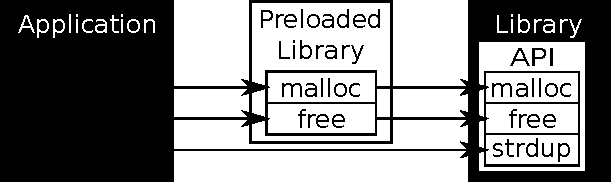
\includegraphics[width=0.8\textwidth]{interception}
  \end{center}
  Famous Example: \textbf{Intel}'s
  \href{https://github.com/intel/opencl-intercept-layer}{\color{blue}
  \underline{Intercept Layer for OpenCL Applications}}
}

\frame{
  \frametitle{Library Interception: Limitations}
  Several limitations come with interception:
  \begin{itemize}
  \item Intercepting calls depends on platform specific functionalities,
  \item Chaining interception libraries can prove difficult if they don't follow
        the same protocol,
  \item Depending on the methods used, there can be quite a lot of boiler-plate
        code involved.
  \end {itemize}
  \textbf{Can we alleviate some of these issues?}
}

\frame{
  \frametitle{Layers as Plugins}
  \textbf{What if this interception could be provided as a plugin by the library
          itself?}

  Examples: Layers for the Vulkan API, PMPI, OMPT, ...
  \begin{block}{Benefits}
    \begin{itemize}
      \item Factoring of platform specific concerns,
      \item Factoring of boilerplate code,
      \item Clear protocol to load layers,
      \item Standardized API for layer development.
    \end{itemize}
  \end{block}
  Design and implement \textbf{Layers for OpenCL}.
  
}

\section{Design and Implementation}

\frame{
  \frametitle{Design and Implementation}
  \begin{center}
  How does the OpenCL \textit{Installable Client Driver} (ICD) Loader work?
  \end{center}
}

\subsection[API Call]{Original OpenCL ICD Loader API Call Workflow}

\frame{
  \frametitle{Original OpenCL ICD Loader API Call Workflow}
  The OpenCL ICD loader is a router for OpenCL calls, directing them to the
correct vendor driver:
  \begin{center}
  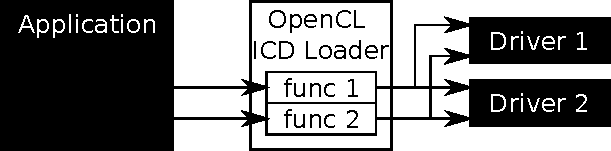
\includegraphics[width=0.8\textwidth]{ICD_Loader}
  \end{center}
}

\begin{frame}[fragile]
  \frametitle{In the Beginning Was the Dispatch Table...}
  In order to support several implementations simultaneously, OpenCL Object are
  required to conform to this definition:
  \tiny
  \begin{minted}[linenos]{c}
/* Dispatch table providing pointers to vendor
 * implementation of the OpenCL API
 */
typedef struct _cl_icd_dispatch {
  /* OpenCL 1.0 */
  cl_api_clGetPlatformIDs clGetPlatformIDs;
  cl_api_clGetPlatformInfo clGetPlatformInfo;
  cl_api_clGetDeviceIDs clGetDeviceIDs;
  cl_api_clGetDeviceInfo clGetDeviceInfo;
  /* ... */
}
struct _cl_device_id { cl_icd_dispatch *dispatch; };
typedef struct _cl_device_id *cl_device_id;
\end{minted}
  \normalsize
  Objects carry around references (function pointers) to the functions (API
  entry points) that need to be used with those objects.
\end{frame}

\begin{frame}[fragile]
  \frametitle{Original OpenCL Loader API Dispatch Example}
  The OpenCL ICD Loader's job is to:
  \begin{itemize}
    \item check for \textit{NULL} handle,
    \item call the correct function in the dispatch table.
  \end{itemize}
  \tiny
  \begin{minted}[linenos]{c}
cl_int clGetDeviceInfo(cl_device_id device,
   cl_device_info param_name, size_t param_value_size,
   void* param_value, size_t* param_value_size_ret)
{
  if (!device) return CL_INVALID_DEVICE;
  return device->dispatch->clGetDeviceInfo(device,
    param_name, param_value_size,
    param_value, param_value_size_ret);
}
\end{minted}
\end{frame}

\subsection[Layer API Call]{OpenCL ICD Loader with Layers API Call Workflow}

\frame{
  \frametitle{OpenCL ICD Loader with Layers API Call Workflow}
  With layer support enabled, the OpenCL ICD loader will:
  \begin{itemize}
  \item first redirect calls to the different active layers,
  \item then dispatch the call to the correct vendor driver.
  \end{itemize}
  \begin{center}
  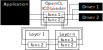
\includegraphics[width=0.8\textwidth]{ICD_Loader_Layers}
  \end{center}
}

\subsection[Implementation]{Loader Layers Implementation}

\frame{
  \frametitle{Loader Layers Implementation Idea}
  How can this scheme be implemented?
  \begin{block}{Constraints:}
    \begin{itemize}
    \item No undue overhead when Layers are not used,
    \item Chain as many layers as required,
    \item Layers should be easy to write and understand.
    \end{itemize}
  \end{block}
  \begin{block}{Idea (layer side):}
    \begin{itemize}
    \item Layers will be given a complete dispatch table to call into,
    \item Any OpenCL call a layer will make will have to be through this table,
    \item Layers will provide a (potentially incomplete) dispatch table of the
          functions they implement to the loader.
    \end{itemize}
  \end{block}
}

\frame{
  \frametitle{Layers Implementation Idea Continued}
  \begin{block}{Idea (loader side):}
    \begin{itemize}
    \item The loader will maintain a list of successfully loaded layers,
    \item Each new layer is added to the front of the list,
    \item Each layer is passed the previous layer dispatch table as a target, or
          the loader internal dispatch table if it is the first,
    \item Incomplete layer tables are completed with their target entries.
    \end{itemize}
  \end{block}
}

\frame{
  \frametitle{Loader Layers Implementation Illustration}
  \begin{figure}
  \centering
  \includegraphics<1>{ICD_Loader_Layer_Loading}%
  \includegraphics<2>{ICD_Loader_Layer_Loading2}%
  \includegraphics<3>{ICD_Loader_Layer_Loading3}%
  \end{figure}
}

\begin{frame}[fragile]
  \frametitle{Original OpenCL Loader API Dispatch Example}
  The OpenCL ICD Loader's job is now to:
  \begin{itemize}
    \item check \textit{if} there are layers, and \textit{then} forward to the
          first layer,
    \item \textit{else}, check for \textit{NULL} handle and call the correct
          function in the dispatch table.
  \end{itemize}
  \tiny
  \begin{minted}[linenos]{c}
cl_int clGetDeviceInfo(cl_device_id device,
   cl_device_info param_name, size_t param_value_size,
   void* param_value, size_t* param_value_size_ret)
{
  if (khrFirstLayer)
    return khrFirstLayer->dispatch.clGetDeviceInfo(
      device, param_name, param_value_size,
      param_value, param_value_size_ret);
  if (!device) return CL_INVALID_DEVICE;
  return device->dispatch->clGetDeviceInfo(device,
    param_name, param_value_size,
    param_value, param_value_size_ret);
}
\end{minted}
\normalsize
The cost of layers when there is no active layer is 1 pointer check.
\end{frame}

\section{Layer Development and Usage}

\frame{
  \frametitle{Layer Development and Usage}
}

\subsection[Layer API]{OpenCL Layers Plugin API}

\frame{
  \frametitle{OpenCL Layer Plugin}
  \begin{itemize}
    \item An OpenCL layer plugin is a shared library,
    \item It must export 2 function symbols:
    \begin{itemize}
      \item \texttt{clGetLayerInfo}
      \item \texttt{clInitLayer}
    \end{itemize}
    \item \textbf{\texttt{clGetLayerInfo}} is used to query information about
          the layer, for now it is limited to the version of the layer API that
          is supported,
    \item \textbf{\texttt{clInitLayer}} is used to negotiate between the loader
          and the layer and exchange dispatch tables. Especially, if the loader
          dispatch table is too small, the layer can refuse to initialize.
    \item The formal extension is called \texttt{cl\_loader\_layers} and can be
          found here: \color{blue}
  \underline{\href{https://github.com/KhronosGroup/OpenCL-Docs/blob/master/ext/cl_loader_layers.asciidoc}{cl\_loader\_layers.asciidoc}}
  \end{itemize}
}

\begin{frame}[fragile]
  \frametitle{\texttt{clGetLayerInfo} API}
\tiny
  \begin{minted}[linenos]{c}
typedef cl_uint cl_layer_info;
typedef cl_uint cl_layer_api_version;
#define CL_LAYER_API_VERSION        0x4240
#define CL_LAYER_API_VERSION_100 100
cl_int clGetLayerInfo(cl_layer_info  param_name,
                      size_t         param_value_size,
                      void          *param_value,
                      size_t        *param_value_size_ret);
\end{minted}
\begin{itemize}
\scriptsize
\item \texttt{param\_name}: Name of the requested parameter (e.g. \texttt{CL\_LAYER\_API\_VERSION})
\item \texttt{param\_value\_size}: Size in bytes of memory pointed to by \texttt{param\_value}
\item \texttt{param\_value}: Pointer to the variable where the info should be stored
\item \texttt{param\_value\_size\_ret}: Optional pointer to a variable to query the info size
\end{itemize}
\scriptsize
\texttt{Returns}:
\begin{itemize}
\scriptsize
\item \texttt{CL\_SUCCESS} on success
\item \texttt{CL\_INVALID\_VALUE} if \texttt{param\_name} is not one of the supported values or if size in bytes specified by \texttt{param\_value\_size} is \texttt{<} size of return type and \texttt{param\_value} is not a NULL value.
\end{itemize}
\end{frame}

\begin{frame}[fragile]
\frametitle{\texttt{clGetLayerInfo} API Implementation}
\tiny
\inputminted[linenos,firstline=8,lastline=31]{c}{example_layer.c}
\end{frame}

\begin{frame}[fragile]
  \frametitle{\texttt{clInitLayer} API}
\tiny
  \begin{minted}[linenos]{c}
cl_int clInitLayer(cl_uint                 num_entries,
                   const cl_icd_dispatch  *target_dispatch,
                   cl_uint                *num_entries_ret,
                   const cl_icd_dispatch **layer_dispatch_ret);
\end{minted}
\begin{itemize}
\scriptsize
\item \texttt{num\_entries}: number of entries in the dispatch table provided by the loader
\item \texttt{target\_dispatch}: pointer to the dispatch table, provided by the loader, that the layer must redirect it’s call to
\item \texttt{num\_entries\_ret}: address to store the number of entries in the layer dispatch table
\item \texttt{layer\_dispatch\_ret}: address to store the pointer to the layer dispatch table
\end{itemize}
\scriptsize
\texttt{Returns}:
\begin{itemize}
\scriptsize
\item \texttt{CL\_SUCCESS} on success
\item \texttt{CL\_INVALID\_VALUE} if \texttt{num\_entries} is insufficient for the layer or if \texttt{target\_dispatch} is a \texttt{NULL} value, or \texttt{num\_entries\_ret} is a \texttt{NULL} value, or \texttt{layer\_dispatch\_ret} is a \texttt{NULL} value.
\end{itemize}
\end{frame}

\begin{frame}[fragile]
\frametitle{\texttt{clInitLayer} API Implementation}
\tiny
\inputminted[linenos,firstline=33,lastline=53]{c}{example_layer.c}
\end{frame}

\begin{frame}[fragile]
\frametitle{simple wrapper}
Display parameters and results of \texttt{clGetPlatformIDs}. Initialize the layer dispatch table.
\tiny
\inputminted[linenos,firstline=55]{c}{example_layer.c}
\normalsize
This covers the bare minimum code required to create a layer.
\end{frame}

\begin{frame}[fragile]
\end{frame}


\subsection[configuration]{OpenCL ICD Loader Layers Configuration Options}

\frame{
  \frametitle{OpenCL ICD Loader Layers Configuration Options}
}

\section[Conclusion]{Conclusion and Perspectives}

\frame{
  \frametitle{Conclusion and Perspectives}
}

\frame{
  \frametitle{Acknowledgement}
  This research used resources of the Argonne Leadership Computing Facility,
  which is a DOE Office of Science User Facility supported under Contract
  DE-AC02-06CH11357.
}

\end{document}
